%%
% Please see https://bitbucket.org/rivanvx/beamer/wiki/Home for obtaining beamer.
%%
%\documentclass[11pt,aspectratio=169]{beamer}
%\documentclass[11pt,aspectratio=169,xcolor={dvipsnames}]{beamer}

\documentclass[11pt,aspectratio=169,xcolor={dvipsnames},hyperref={pdftex,pdfpagemode=UseNone,hidelinks,pdfdisplaydoctitle=true},usepdftitle=false]{beamer}
\usepackage{presentation}


\title{Lecture 9: Price Rigidity and Menu Cost Models}
\author{Juan Herre\~{n}o\\UCSD}
\date{2026}

% Enter presentation title to populate PDF metadata:
\newcommand{\Cov}{\text{Cov}_\lambda}
\newcommand{\El}{\mathbb{E}_\lambda}
\newcommand{\mm}{\text{{\fontfamily{qzc}\selectfont m}}}
\usepackage{cancel}
\usepackage{booktabs}
\begin{document}

\maketitle


\begin{frame}{Start with Basic Facts}
\begin{itemize}
\item How often do price setters change prices?
\item Older literature from the 1990s looked at very particular prices
\begin{itemize}
\item Examples: Prices of newspapers. Retail prices in a particular supermarket.
\end{itemize}
\item Bils and Klenow (2004) use price change reports from the BLS
\begin{itemize}
\item Covers roughly 70\% of consumer expenditures
\item  Average duration of a price is roughly 4-5 months
\item Suggests a frequency of price change of 20\%
\item Average absolute change of price changes is large (10\%).
\end{itemize}
\item Back of the envelope calculation
\begin{itemize}
\item If 20\% of prices change by 10\% every month. Does that suggest an inflation rate of 2\% per month?
\item Clearly not. CPI inflation in the USA is roughly 2\% \textbf{per year}
\item It must be that there are price increases and decreases at the same time
\item Textbook Calvo model doesn't get this right. No role for idiosyncratic price changes
\end{itemize}
\end{itemize}
\end{frame}

\begin{frame}{What is a price change}
\begin{itemize}
\item Above back-of-the-envelopes assumed ``a price change is a price change''
\item But some empirical issues
\begin{itemize}
\item How do we treat temporary sales?
\item How do we treat seasonal price changes?
\item How do we treat substitutions?
\item Are all prices selected as a function of the \textbf{macro} environment?
\end{itemize}
\item Big picture. We are interested in how macroeconomic policy induces price changes
\item What matters is how sluggish is aggregate $P$ to changes in aggregate demand
\end{itemize}
\end{frame}

\begin{frame}{An example}
\begin{figure}
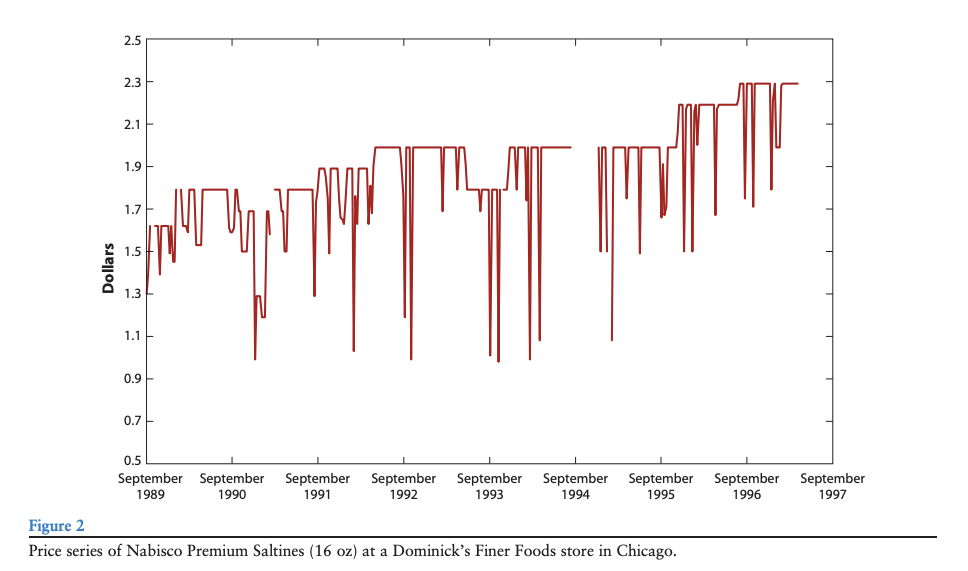
\includegraphics[scale=0.35]{FiguresTables/ns2013_1}\\
Source: Nakamura and Steinsson (2013)
\end{figure}
\end{frame}

\begin{frame}{An example}
\begin{itemize}
\item Sales are frequent and large
\item Regular price changes are lumpy and infrequent
\item Is this price essentially flexible (117 price changes in 365 weeks)?
\item Or essentially rigid (9 regular price changes over 7 years)?
\end{itemize}
\end{frame}

\begin{frame}{Beyond an Example}
\begin{figure}
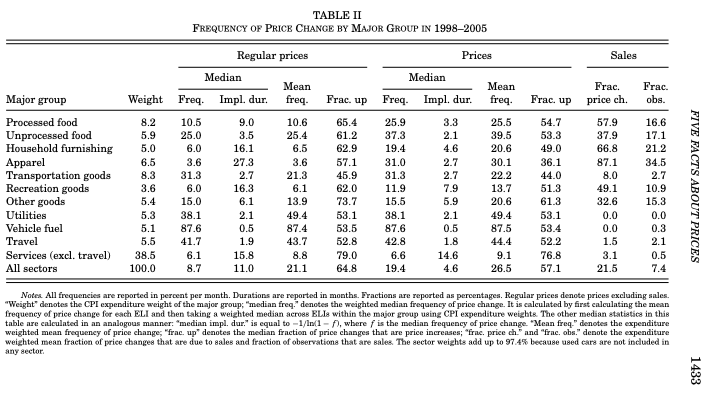
\includegraphics[scale=0.5]{FiguresTables/ns2008_1}\\
Source: Nakamura and Steinsson (2008)
\end{figure}
\end{frame}



\begin{frame}{Sales seem special. CPI vs. PPI}
\begin{figure}
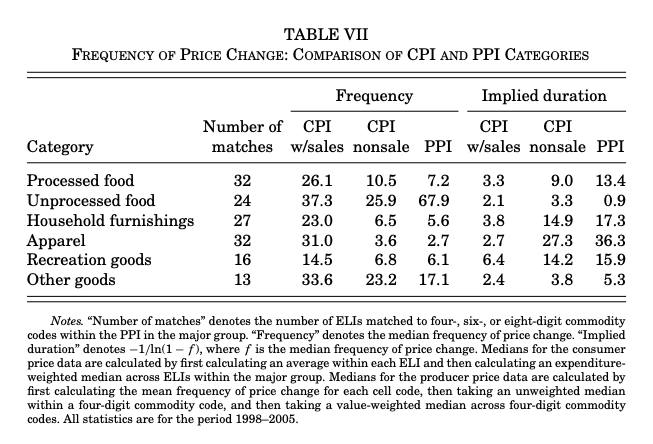
\includegraphics[scale=0.4]{FiguresTables/ns2008_2}\\
Source: Nakamura and Steinsson (2008)
\end{figure}
\end{frame}


\begin{frame}{Price changes are large and plenty in both directions}
\begin{figure}
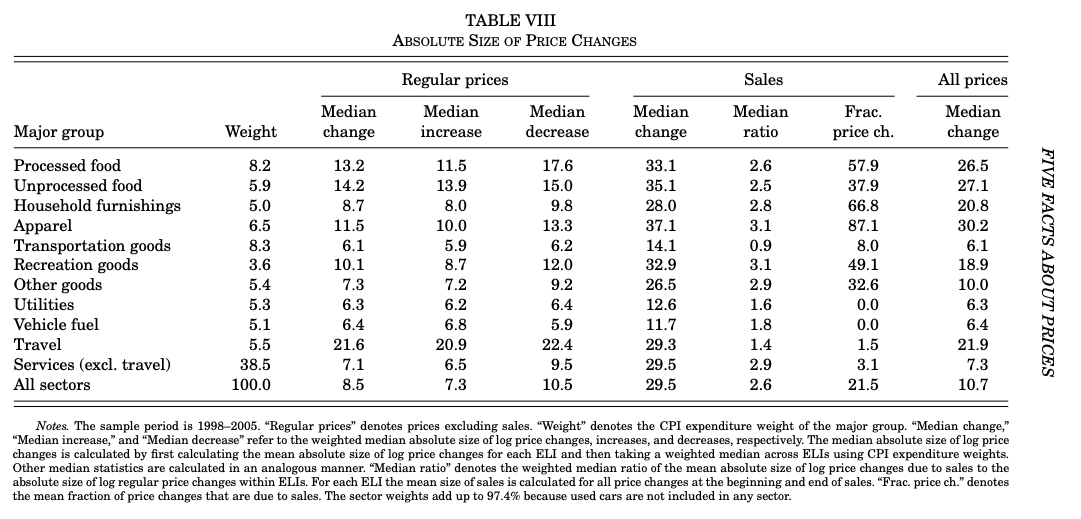
\includegraphics[scale=0.35]{FiguresTables/ns2008_3}\\
Source: Nakamura and Steinsson (2008)
\end{figure}
\end{frame}

\begin{frame}{Frequency of adjustment comoves with inflation - USA}
\begin{figure}
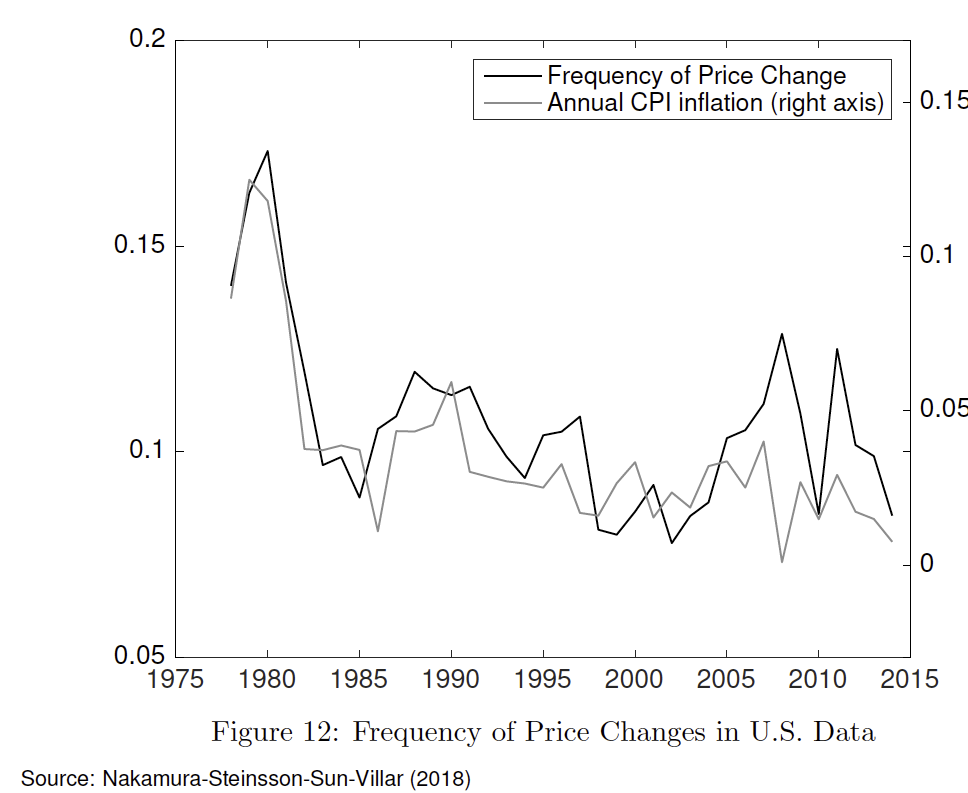
\includegraphics[scale=0.25]{FiguresTables/nssv}\\
\end{figure}
\end{frame}



\begin{frame}{Frequency of adjustment comoves with inflation - Mexico}
\begin{figure}
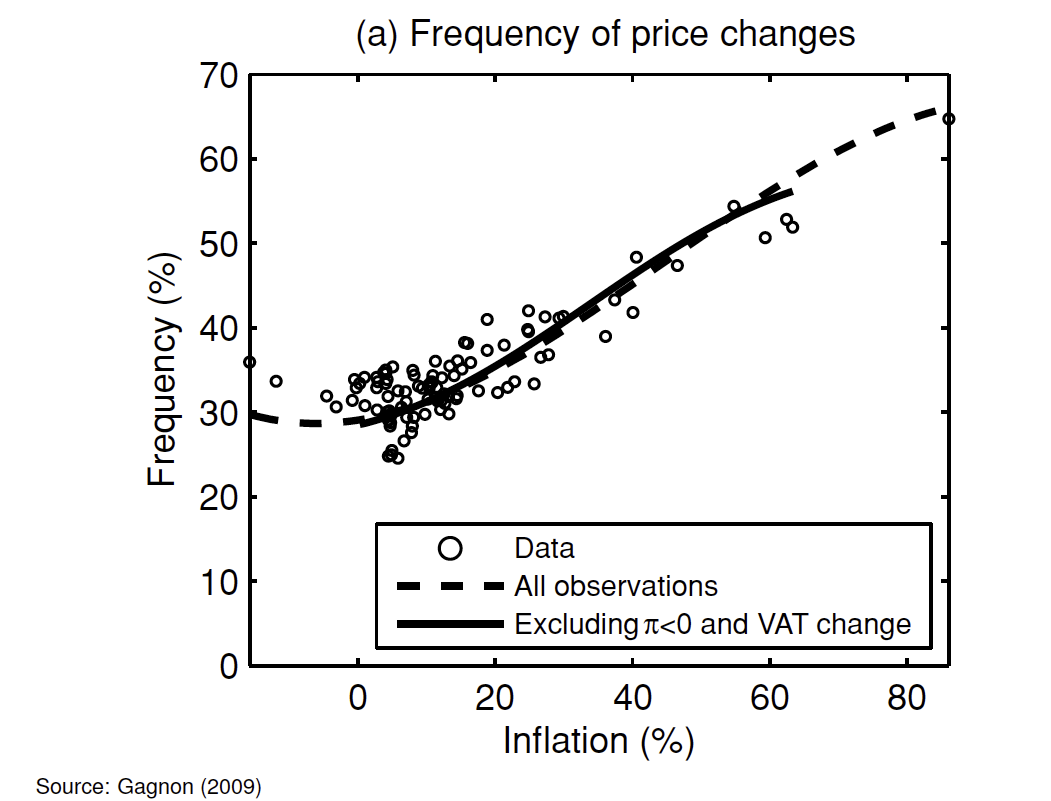
\includegraphics[scale=0.25]{FiguresTables/gagnon_1}\\
\end{figure}
\end{frame}

\begin{frame}{Frequency of adjustment comoves with inflation - Mexico}
\begin{figure}
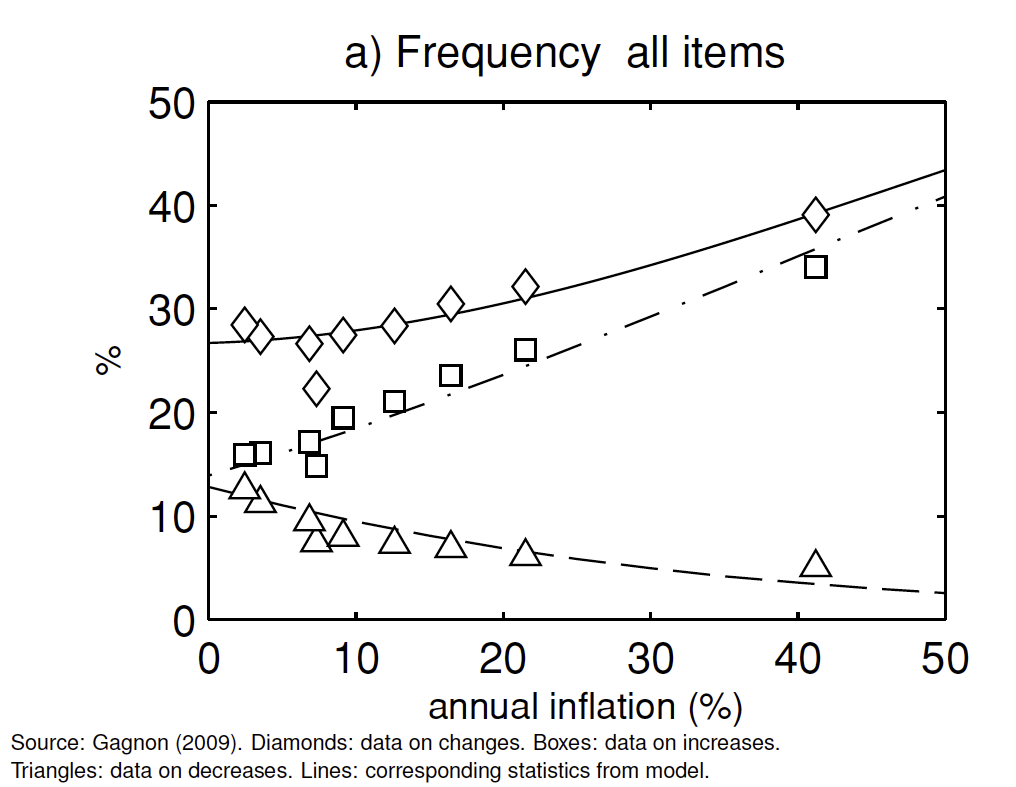
\includegraphics[scale=0.25]{FiguresTables/gagnon_2}\\
\end{figure}
\end{frame}

\begin{frame}{Frequency of adjustment comoves with inflation - Argentina}
\begin{figure}
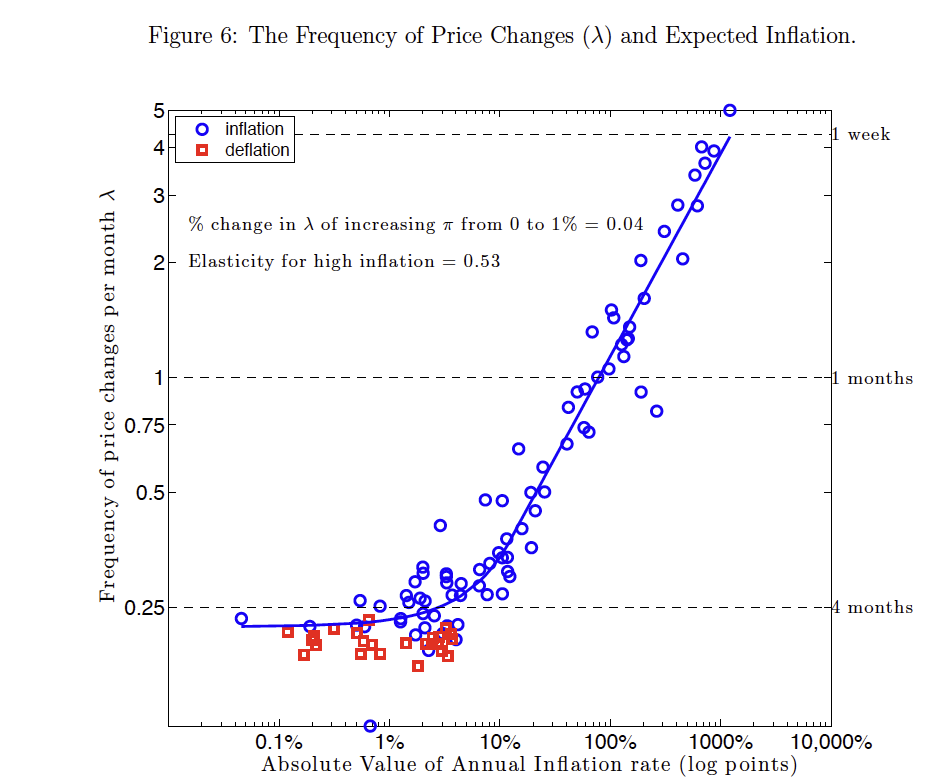
\includegraphics[scale=0.25]{FiguresTables/abn_1}\\
\end{figure}
\end{frame}

\begin{frame}{Many arrows point in the same direction}
\begin{itemize}
\item Remember in Calvo only one invariant parameter mattered: the frequency of price changes
\item Perhaps our Calvo model is ``too simple''
\item Some reasons:
\begin{itemize}
\item The frequency of price changes comoves with inflation
\item The share of price increases vs. price decreases moves with inflation
\item Absolute size of price changes does not comove with inflation
\end{itemize}
\item Suggests that:
\begin{itemize}
\item Maybe price resetters are ``selected'' (i.e., not a random sample of firms)
\item This issue in the literature is called ``the selection effect''
\end{itemize}
\end{itemize}
\end{frame}

\begin{frame}{Caplin-Spulger model}
\begin{itemize}
\item The math is beside the point. It can be explained intuitively.
\item The monetary authority targets nominal GDP (easy to microfound with a central bank that targets the money supply and with a cash-in-advance constraint in the background)
\item In logs, $m_t = y_t + p_t$
\item $m_t$ is increasing, and desired prices are $p^*_t \propto m_t$
\item Firms must pay a fixed cost to change their price
\item When the relative price goes below $s$, firms adjust it to $S$
\item This class of models, which we will specify more formally, is called $sS$ models
\item Initial distribution of firms is uniform $\in [s,S]$.
\end{itemize}
\end{frame}


\begin{frame}{Caplin-Spulger model}
\begin{itemize}
\item Imagine $m$ increases by an amount $\Delta m$
\item Any firm with a relative price below $s + \Delta m$ will adjust (the increase in $m$ puts them below $s$)
\item They all adjust to $S$
\item Share of firms that adjust? Because of the uniform distribution:
$$\frac{\Delta m}{S-s}$$
\item By how much do they adjust?
$$S-s$$
\item Total price change
$$\Delta p = \frac{\Delta m}{S-s} S-s = \Delta m$$
\item Change in total output?
$$\Delta y = \Delta m - \Delta p = 0$$
\item Money is neutral!
\end{itemize}
\end{frame}

\begin{frame}{Calvo vs. Caplin Spulberg}
\begin{itemize}
\item In Calvo, firms that adjust their prices are chosen at random
\item These may be firms that do not need to adjust their prices by much
\item Many price adjustments are ``wasted'' in firms that adjust little when given the chance
\item So the aggregate price level moves slowly
\item In Caplin and Spulberg firms that change their price are firms that need to reset the most
\item The aggregate price level moves rapidly
\end{itemize}
\end{frame}


\begin{frame}{Calvo vs. Caplin-Spulberg}
\begin{itemize}
\item Both models are extremes
\item Calvo
\begin{itemize}
\item Aggregate conditions have no effect on the share or the identity of firms that adjust
\end{itemize}
\item Caplin Spulberg
\begin{itemize}
\item Fully determine which, and how many firms adjust
\item Other very special assumptions (uniform initial distribution), $\Delta m$ shocks do not alter the uniform distribution are very important
\end{itemize}
\end{itemize}
\end{frame}

\begin{frame}{Golosov Lucas 07 (modified)}
\begin{itemize}
\item Household prefereces (log + linear)
$$\mathbb{E}_0 \sum \beta^t \left( \log C_t - \omega L_t \right)$$
\item $C$ a CES aggregator
$$C_t = \left(\int c_t(z)^{\frac{\theta-1}{\theta}} dz \right)^{\frac{\theta}{\theta-1}}$$
\item subject to a series of budget constraints
$$P_t C_t + Q_{t+1} B_{t+1} \leq W_t L_t + \int \Pi_t(z) dz$$
\end{itemize}
\end{frame}

\begin{frame}{Household optimization}
Very standard. Special case of our previous models
\begin{align}
c_t(z) = C_t \left(\frac{p_t(z)}{P_t}\right)^{-\theta}\\
W_t = \omega P_t C_t
\end{align}
Notice that the real wage is proportional to consumption
\end{frame}


\begin{frame}{Monetary policy}
\begin{itemize}
\item Similar than in the simple Caplin Spulberg model
\begin{align}
S_t = P_t C_t
\end{align}
\item Central bank sets the money supply according to
\begin{align}
\log S_t = \mu \log S_{t-1} + \eta_t
\end{align}
\item for $\eta$ distributed $N(0,\sigma^2_\eta)$
\item $\eta$ is the only aggregate shock
\end{itemize}
\end{frame}


\begin{frame}{Firm's problem}
\begin{itemize}
\item Linear production function on labor with idiosyncratic productivity shocks
$$y_t(z) = A_t(z) L_t(z)$$
\item Marginal cost of production is $W_t/A_t(z)$
\item $\log A_t(z)  = \rho \log A_{t-1}(z) + \epsilon_t(z)$, for $\epsilon$ distributed $N(0,\sigma^2_{\epsilon}$ 
\end{itemize}
\end{frame}

\begin{frame}{Firm's problem}
\begin{itemize}
\item Maximize NPV of dividends
$$\mathbb{E}_t \sum_{k=0}^{\infty} \Lambda_{t,t+k}\Pi_{t}(z)$$
\item where profits are
$$\Pi_t(z) = p_t(z) y_t(z) - W_t L_t(z) - \chi_j W_t I_t(z)$$
\item Hire $\chi_j$ units of labor to change prices
\item $\Lambda$ the SDF
\end{itemize}
\end{frame}

\begin{frame}{Fixed cost}
\begin{itemize}
\item Cannot log-linearize this problem. Kink because of fixed costs.
\item Must go with dynamic programming
$$V(Z_t) = \max_{p_t} \Pi^R_t(z) + \mathbb{E}(\Lambda^R_{t,t+1}V(Z_{t+1})$$
\item where $\Pi^R(z) = C_t\left(\frac{p_t(z)}{P_t}\right)^{-\theta} \left(\frac{p_t(z)}{P_t} - \frac{1}{A_t(z)}\frac{W_t}{P_t} \right) - \chi_j \frac{W_t}{P_t}I_t(z)$
\item $Z_t$ are the state variables. What are the state variables?
\item In general: everything that affects firms's value
\item $A_t(z), p_{t-1}(z)/P_t, C_t$  
\item Any variable that you need to forecast $C_{t+1}, P_{t+1}$
\item So you need the entire distribution of $A_t(z), p_{t-1}(z)/P_t$
\end{itemize}
\end{frame}

\begin{frame}
\begin{figure}
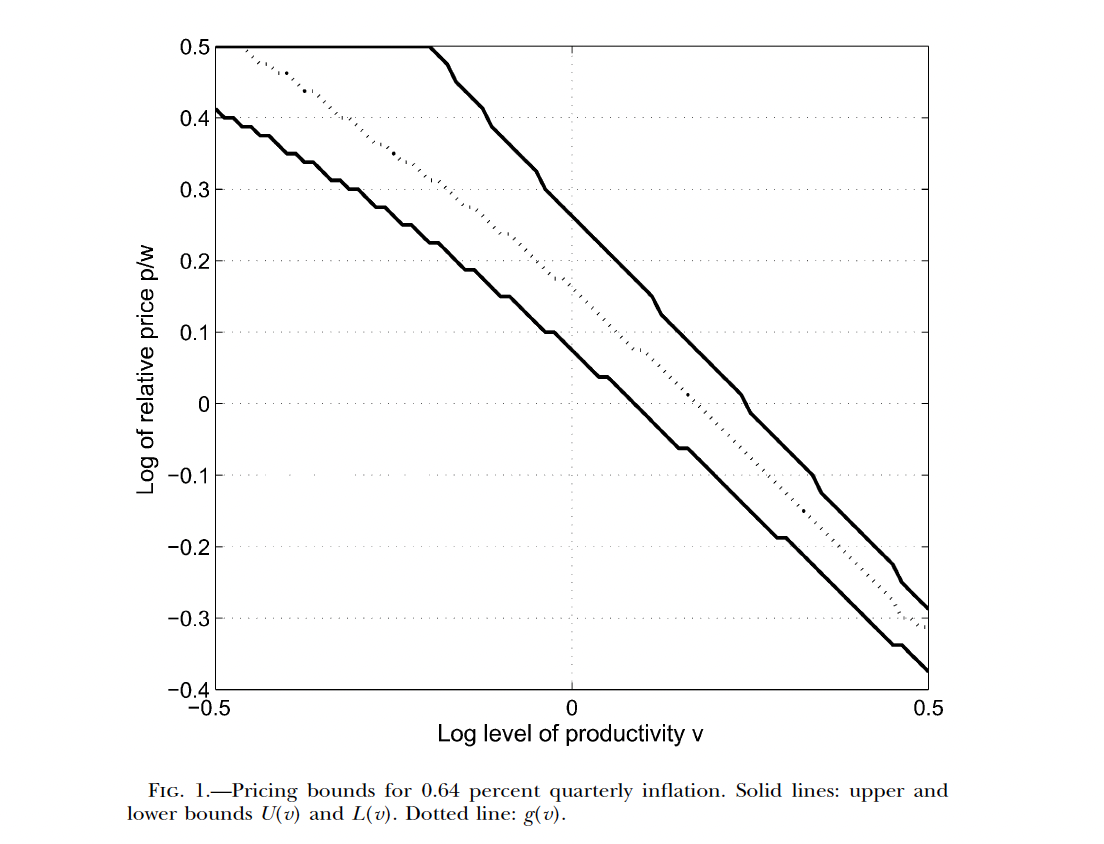
\includegraphics[scale=0.45]{FiguresTables/gs_1}\\
Source: Golosov and Lucas (2007)
\end{figure}
\end{frame}

\begin{frame}
\begin{figure}
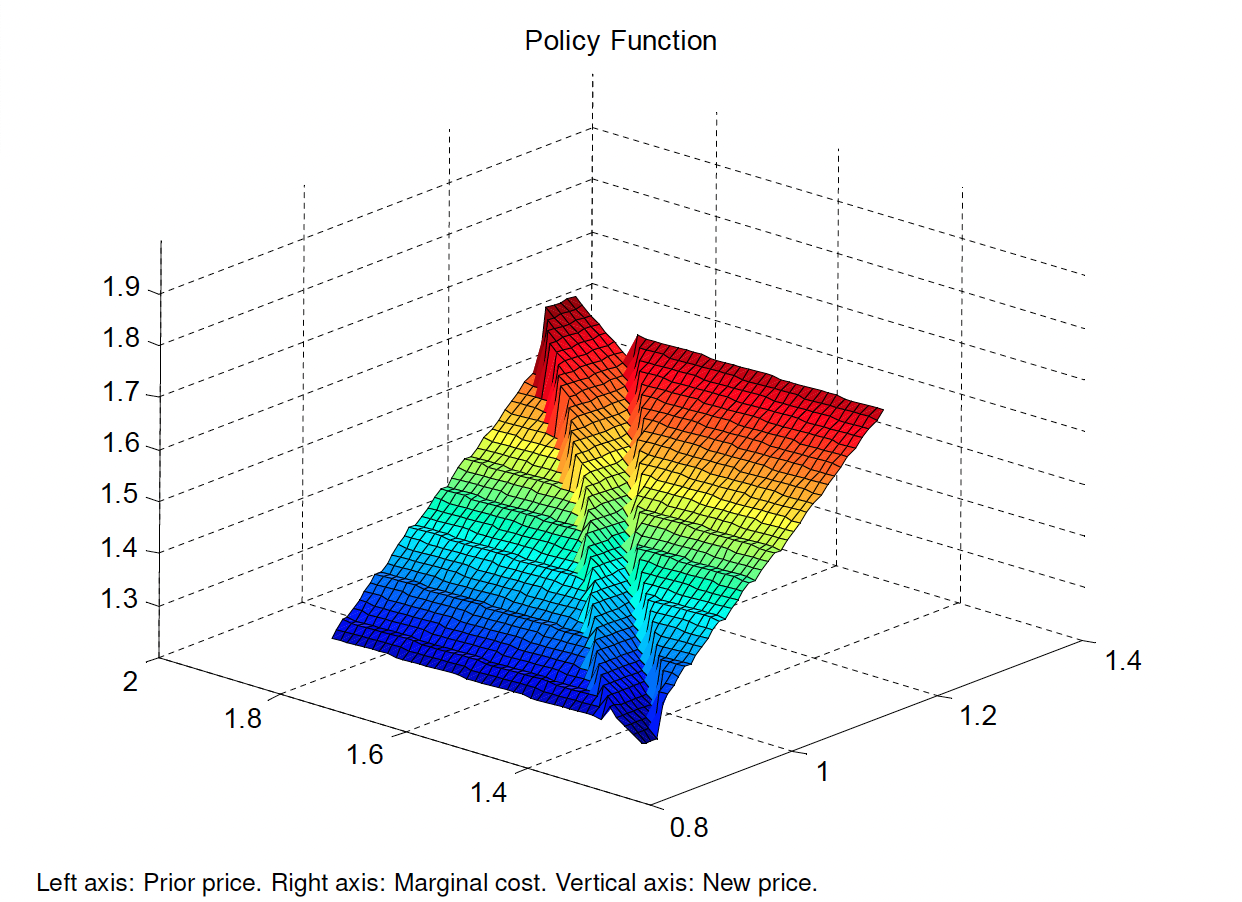
\includegraphics[scale=0.45]{FiguresTables/gs_2}\\
Source: Golosov and Lucas (2007)
\end{figure}
\end{frame}


\begin{frame}
\begin{figure}
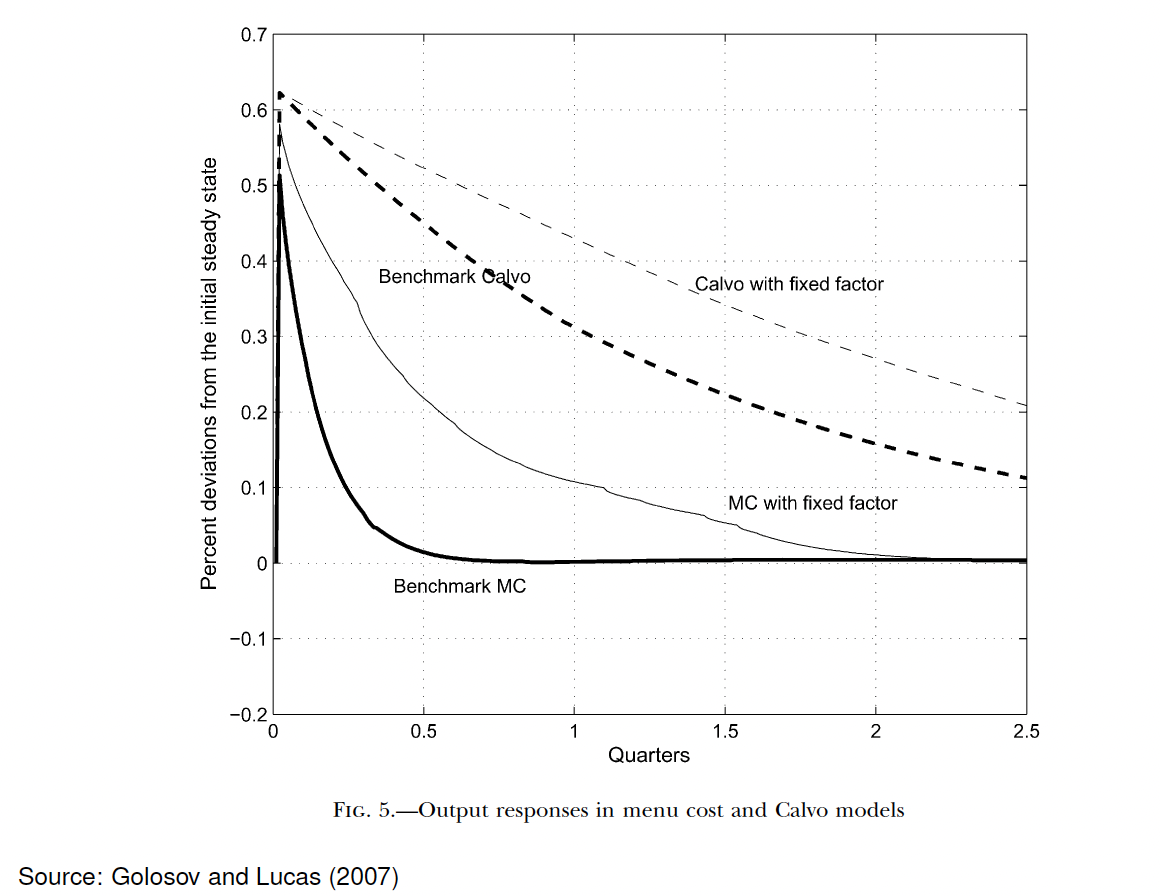
\includegraphics[scale=0.45]{FiguresTables/gs_3}\\
Source: Golosov and Lucas (2007)
\end{figure}
\end{frame}

\begin{frame}
\begin{figure}
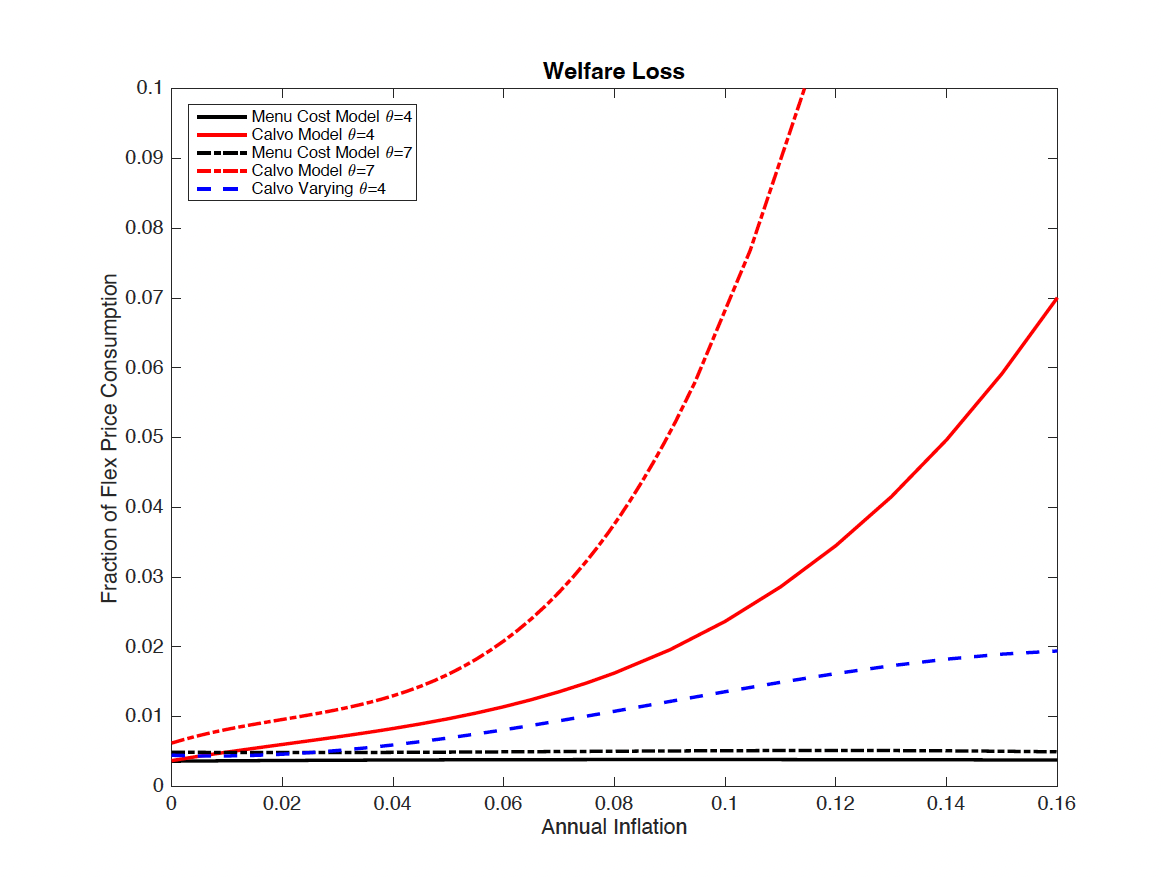
\includegraphics[scale=0.45]{FiguresTables/ns2010_10}\\
Source: Nakamura Steinsson Sun Villar (2018)
\end{figure}
\end{frame}

\begin{frame}{Issues with Golosov Lucas (2007)}
\begin{itemize}
\item Calibrated using Bils Klenow numbers
\item Golosov and Lucas (2007): Monetary non-neutrality is small and transient. But!
\begin{itemize}
\item Remember our discussion about regular vs. sales.
\item Abstracts from sectoral heterogeneity in price rigidity. Paula will talk how important this is
\item Odd predictions about the distribution of price changes (see next slide)
\item Once ``fixed'' menu cost model waaay closer to Calvo
\item But we saw Calvo fails in many dimensions too!
\end{itemize}
\end{itemize}
\end{frame}


\begin{frame}
\begin{figure}
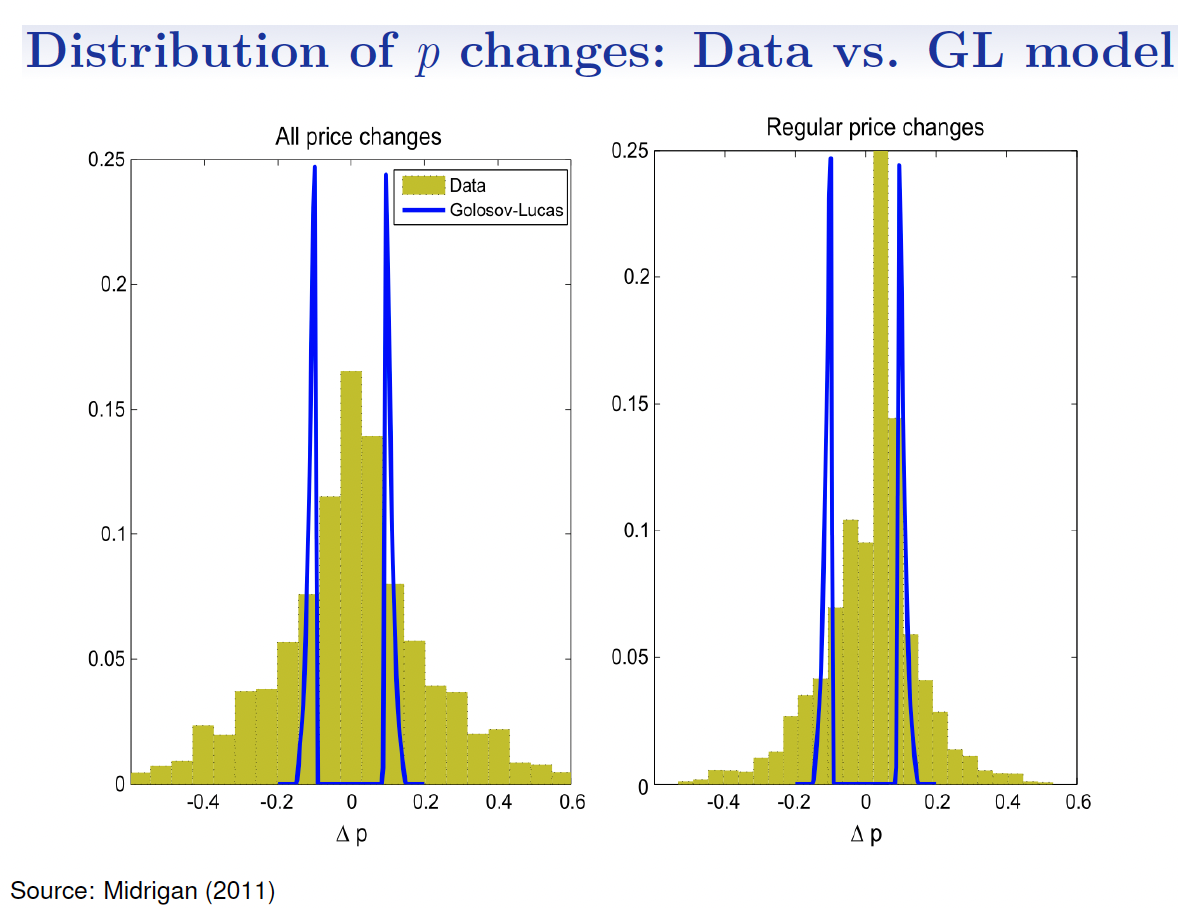
\includegraphics[scale=0.45]{FiguresTables/midrigan}\\
Source: Midrigan (2011)
\end{figure}
\end{frame}


\end{document}




